\documentclass{article}

% Langue
\usepackage[utf8]{inputenc}
\usepackage[T1]{fontenc}      
\usepackage[francais]{babel}

% Mise en forme générale
\usepackage[top=2.5cm,bottom=2.5cm,right=2.5cm,left=2.5cm]{geometry}

% Package divers
\usepackage{chemist} 
\usepackage[version=3]{mhchem}
\usepackage{chemfig}
\usepackage[squaren, Gray]{SIunits}
\usepackage{sistyle}
\usepackage[autolanguage]{numprint}
\usepackage{url}
\usepackage{rotating}
\usepackage{xcolor,colortbl}
\definecolor{Gray}{gray}{0.85}

\usepackage{hyperref}
\hypersetup{
    colorlinks,
    citecolor=black,
    filecolor=black,
    linkcolor=black,
    urlcolor=black
}

% Nouvelles commandes
\newcommand{\std}{\ensuremath{^{\circ}}}
\newcommand\ph{\ensuremath{\mathrm{pH}}}
\newcommand{\annexe}{\part{Annexes}\appendix}
\newcommand{\biblio}[1]{\bibliographystyle{plain}\bibliography{#1}\nocite{*}}

\newcommand{\doctitle}[1]{
	\title{#1}
	\author{\textbf{Groupe 124.3}\\
	\textsc{Frenyo} Péter (6266-12-00)\\
	\textsc{Gillain} Nathan (7879-12-00)\\
	\textsc{Lamine} Guillaume (7109-13-00)\\
	\textsc{Piraux} Pauline (2520-13-00)\\
	\textsc{Paris} Antoine (3158-13-00)\\
	\textsc{Quiriny} Simon (4235-13-00)\\
	\textsc{Schrurs} Sébastien (7978-13-00)}
	\date{\today}

	\begin{document}

	\maketitle
	\tableofcontents
}

%\usepackage[version=3]{mhchem} surement deja utilise mais au cas ou
\doctitle{Conception plus détaillée de la dernière étape du procédé :
la synthèse d'ammoniac proprement dite}

\section{Etude thermodynamique}
Nous avions d'abord fait l'hypothèse que la synthèse était complète.
Nous pouvons maintenant l'analyser plus en détails en la considérant
à l'équilibre thermodynamique. Nous ferons ici l'hypothèse du gaz
parfait, une étude plus rigoureuse à l'aide du logiciel \textsc{Aspen+}
sera faite par la suite. Notons à l'avance que nous travaillerons
à pression constante étant donné que nous sommes dans un système ouvert.
On se rend vite compte qu'une conversion complète n'est pas réalisable. 
Nous avons alors incorporé une boucle de recyclage des réactifs résiduels
afin de les renvoyer à l'entrée du réacteur. Cette boucle comprend une 
purge afin d'éviter l'accumulation d'argon présent dans l'air. 
% FIX : (et une surpression?)

Le tableau~\ref{tab:ammoniac} fait le bilan à l'équilibre thermodynamique.

\begin{table}[!ht]
	\begin{center}
		\begin{tabular}{c|ccc}
			Avancement & 
			\multicolumn{1}{c!{\makebox[0pt]{+}}}{\ce{1/2N2_{(g)}}} &
			\multicolumn{1}{c!{\makebox[0pt]{$\rightleftharpoons$}}}{\ce{3/2H2_{(g)}}} &
			\ce{NH3_{(g)}} \\
			\hline
			$n_i$ & $n_1$ & $n_2$ & $0$ \\
			$n_{eq}(x)$ & $n_1 - \frac{x}{2}$ & $n_2 - \frac{3x}{2}$ & $x$ \\
			\hline
			$a(x)$ & 
			%$\frac{2n_{1} - x}{2 n_{g,tot}} \frac{p_{tot}}{p \degree}$ 
			$\frac{2n_{1} - x}{2 n_{g,tot}} \frac{p_{tot}}{p_0}$ &
			$\frac{2n_{2} - 3x}{2 n_{g,tot}} \frac{p_{tot}}{p_0}$ &
			$\frac{x}{n_{g,tot}} \frac{p_{tot}}{p_0}$ \\
		\end{tabular}
		\caption{Tableau d'avancement de la réaction de synthèse de l'ammoniac.}
		\label{tab:ammoniac}
	\end{center}
\end{table}

Dans celui-ci, $n_1$, $n_2$ et $n_3$ sont respectivement les débits molaires 
d'azote, d'hydrogène et d'argon. De plus,la somme des débits molaires de gaz
à l'équilibre est : $n_{g,tot} = n_1 + n_2 + n_3 - x$. 

On retire de cela et du tableau~\ref{tab:ammoniac}, une expression de la constante d'équilibre :

$$K(T) = \frac{4x\cdot p_0\cdot n_{g,tot}}{(2n_1 - x)^{1/2} (2n_2 - 3x)^{3/2} \cdot p_{tot}}.$$

Pour analyser quantitativement la réaction, utilisons le graphe de la figure~\ref{fig:purge}
% FIX : où est la figure?
En développant le problème dans le cas d'un recyclage avec purge, on a :

\begin{align}
	\notag
	\begin{cases}
	 n_1 = \ce{N2_{,in} + N2_{,rec}} \\
	 n_2 = \ce{H2_{,in} + H2_{,rec}} \\
	 n_3 = \ce{Ar_{in} + Ar_{rec}} \\
	\end{cases}
	 &  \text{et}  &
	\begin{cases}
	 \ce{N2_{,syn}} = n_1 - \frac{x}{2} \\
	 \ce{H2_{,syn}} = n_2 - \frac{3x}{2} \\
	 \ce{NH3_{,syn}} = x \\
	 \ce{Ar_{syn} = Ar_{in} + Ar_{rec}} \\ 
	\end{cases}
	\\
\end{align}

Les équations de gauche sont dues au recyclage et celles de droite 
à la conservation de la matière. Ensuite, nous avons les trois relations
de la purge où nous posons un coefficient $k$ de proportion entre ce qui
est recyclé et ce qui sort du réacteur de synthèse. On fait l'hypothèse
que la purge enlève une proportion égale de moles pour chaque composé.

$$
\begin{cases}
 k\cdot \ce{N2_{,syn}} = \ce{N2_{,rec}} \\ 
 k\cdot \ce{H2_{,syn}} = \ce{H2_{,rec}} & k \in [0 \text{(ouvert)}, 1 \text{(fermé)}[ \\
 k\cdot \ce{Ar_{syn}} = \ce{Ar_{rec}} \\
\end{cases}
$$

Enfin, il nous reste à imposer que en régime l'argon rentrant doit être égal
à l'argon purgé. C'est indispensable pour éviter une accumulation du composé
dans le réacteur, et une baisse du rendement. 
Il faut donc : $(1 - k)\ce{Ar_{syn}} = \ce{Ar_{in}}$.

A partir de ces différentes équations, nous pouvons exprimer l'ammoniac
sortant en fonction des composants à l'entrée, du coefficient, de la pression
totale et de la température. Les détails du calcul sont laissés à l'attention 
du lecteur. Nous arrivons finalement à l'équation~\eqref{eq:finale}, qui peut
être résolue numériquement à l'aide de l'outil \textsc{Matlab}.  

\begin{align}
	K(T) & = \frac{4x\cdot p_0\cdot (\ce{N2_{,in} + H2_{,in} + Ar_{in}} - 
	\ce{NH3_{,syn}}(k + 1)) (1 - k)}{(\ce{2N2_{,in} - NH3_{,syn}})^{1/2} (\ce{2H2_{,in} - 3NH3_{,syn}})^{3/2} \cdot p_{tot}}
	\label{eq:finale}
\end{align}

Pour pouvoir complèter notre outil de gestion, nous exprimons les entrées 
en fonction du débit d'ammoniac voulue, de $k$, de la pression et de la
température. Pour cela nous nous plaçons dans le cas idéal stœchiométrique,
où aucuns des composants n'est en excès. De plus, nous prenons en compte la 
concentration d'argon naturellemnt dans l'air. 
 
$$
\begin{cases}
 \ce{N2_{,in}} = \ce{78Ar_{in}}\\ 
 \ce{N2_{,in}} = \ce{3H2_{,in}} \\
\end{cases}
$$

\section{Utilisation du logiciel \textsc{Aspen+}}
Nous avons ensuite utilisée le logiciel \textsc{Aspen+}
afin de simuler la synthèse de l'ammoniac. Pour cela
nous avons construit le flow-sheet présenté à la figure
\ref{fig:flow-sheet-aspen}. 

\begin{figure}
	\centering
	\rotatebox{90}{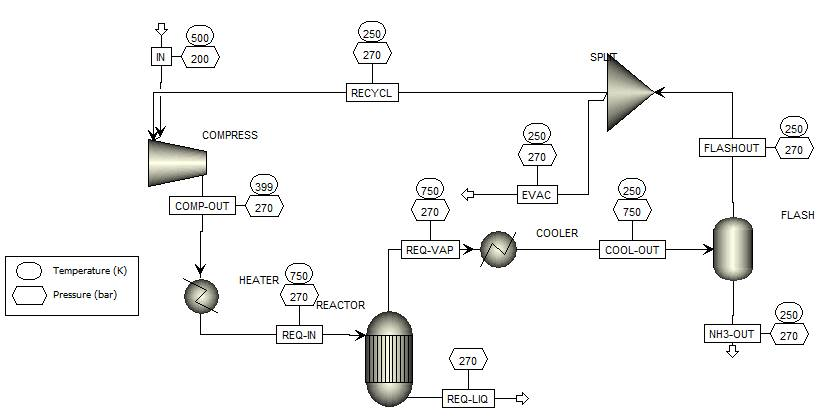
\includegraphics[scale=0.7]{media/flow-sheet.jpg}}
	\caption{Flow-sheet du procédé de synthèse de l'ammoniac
	réalisé avec \textsc{Aspen+}.}
	\label{fig:flow-sheet-aspen}
\end{figure}

% FIX : c'est bien cette méthode là?
Pour la simulation, nous avons utilisé la méthode
thermodynamique \textsc{SRK} qui est particulièrement
approprié pour les réactions entre gaz avec une pression
et une température élevée. Nous avons choisi d'utiliser
une purge de 4\%. La simulation nous fournit les résultats
présente à la figure \ref{fig:resultats-aspen}.

\begin{figure}
	\centering
	\rotatebox{90}{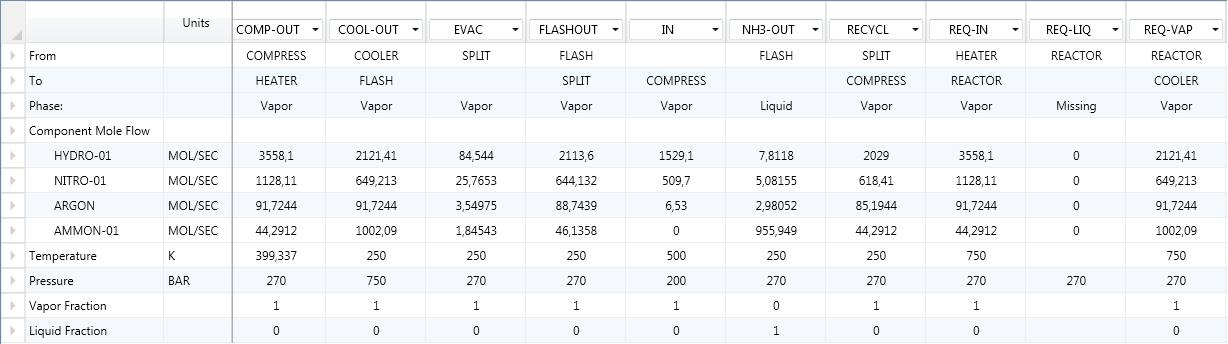
\includegraphics[scale=0.48]{media/results.jpg}}
	\caption{Résultats du procédé de synthèse de l'ammoniac
	réalisé avec \textsc{Aspen+}.}
	\label{fig:resultats-aspen}
\end{figure}

Ces résultats sont assez proches de ceux fournis par
l'outil de gestion. % TODO : erreur à calculer en % pour donner une meilleure idée
\end{document}